We can now analyse separately the results for $h_{11}$ and $h_{21}$ for each considered algorithm. We will compare the naive results using the configuration matrix with the most important scalar feature (\texttt{num\_cp}) and the most important vector feature (\texttt{dim\_cp}) and then use the engineered dataset.

\subsection{Linear Regression}
    We first consider the \texttt{LinearRegression} algorithm. We used a \texttt{GridSearchCV} for the hyperparameters \texttt{fit\_intercept} and \texttt{normalize} and we use the \textit{floor} function for the accuracy.
    
    The naive computation with only the matrix components for $h_{11}$ reached $50.6\% \pm 1.1\%$ of accuracy during cross-validation and $50.8\%$ of accuracy for the test predictions using \texttt{fit\_intercept = False} and \texttt{normalize = True}. The same computation for $h_{21}$ led to $10.8\% \pm 1.6\%$ during cross-validation and $12.3\%$ of accuracy in the test set using \texttt{fit\_intercept = True} and \texttt{normalize = False}.
    
    The baseline computation with \texttt{num\_cp} only for $h_{11}$ reached $62\% \pm 2\%$ of accuracy during cross-validation and $63\%$ of accuracy during the test predictions using \texttt{fit\_intercept = True} and \texttt{normalize = True}, thus showing a major improvement in the predictions with respect to the naive case. For $h_{21}$ things get slightly worse in this case with $8.5\% \pm 0.6\%$ of accuracy in cross-validation and $9.2\%$ for the test set using \texttt{fit\_intercept = True} and \texttt{normalize = True}.
    
    The second baseline computation using only \texttt{dim\_cp} shows a worse result for $h_{11}$ with $43.7\% \pm 1.4\%$ in cross-validation and $44.9\%$ of accuracy for the test predictions with \texttt{fit\_intercept = True} and \texttt{normalize = False}, while the results for $h_{21}$ are stable with $8.4\% \pm 0.9\%$ in cross-validation and $8.3\%$ of accuracy for the test set using \texttt{fit\_intercept = False} and \texttt{normalize = True}.
    
    The complete computation using the engineered features improves both $h_{11}$ and $h_{21}$. Specifically we get $52\% \pm 2\%$ of accuracy in cross-validation for $h_{11}$ and $53\%$ during the test predictions using \texttt{fit\_intercept = True} and \texttt{normalize = True}, while the accuracy for $h_{21}$ is almost doubled with $19.4\% \pm 1.6\%$ of accuracy during cross-validation and $20.6\%$ during the test predictions using \texttt{fit\_intercept = False} and \texttt{normalize = True}. We show in Figure~\ref{fig:lin_reg_err} the distribution of the the errors of the test predictions, that is the signed difference between the true value and the prediction.
    
    \begin{figure}[t]
        \centering
        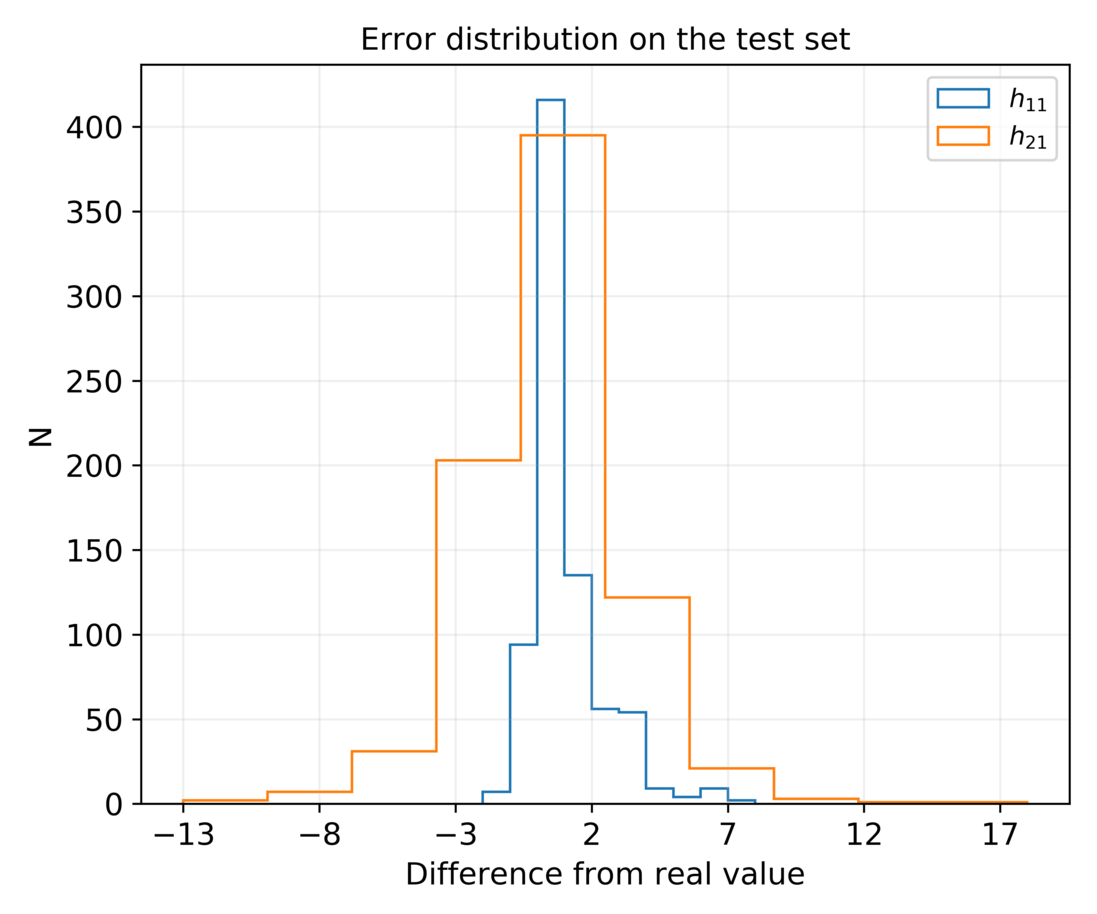
\includegraphics[width=0.75\textwidth]{tex/img/lin_reg_error_eng.png}
        \caption{Error distribution for \texttt{LinearRegression} using the engineered dataset.}
        \label{fig:lin_reg_err}
    \end{figure}
    
\subsection{Lasso Regression}
    We then consider the \texttt{Lasso} algorithm which implements $l1$-regularization with respect to the linear regression algorithm. We implement a search space for the \texttt{BayesSearchCV} for the hyperparameters \texttt{alpha}, \texttt{fit\_intercept}, \texttt{normalize} and \texttt{positive} and we use the \textit{floor} function for the accuracy.
    
    The naive computation with only the matrix components for $h_{11}$ reached $51.0\% \pm 1.6\%$ of accuracy during cross-validation and $50.4\%$ of accuracy for the test predictions using \texttt{alpha = $8.0 \times 10^{-5}$}, \texttt{fit\_intercept = False}, \texttt{normalize = True} and \texttt{positive = True}. The same computation for $h_{21}$ led to $11.4\% \pm 1.1\%$ during cross-validation and $11.5\%$ of accuracy in the test set using \texttt{alpha = $2.6 \times 10^{-4}$}, \texttt{fit\_intercept = True}, \texttt{normalize = True} and \texttt{positive = False}.
    
    The baseline computation with \texttt{num\_cp} only for $h_{11}$ reached $62\% \pm 2\%$ of accuracy during cross-validation and $63\%$ of accuracy during the test predictions using \texttt{alpha = $1.6 \times 10^{-4}$}, \texttt{fit\_intercept = True}, \texttt{normalize = True} and \texttt{positive = False}, thus showing a major improvement in the predictions with respect to the naive case. For $h_{21}$ we find $10.4\% \pm 0.9\%$ of accuracy in cross-validation and $9.8\%$ for the test set using \texttt{alpha = $1.2 \times 10^{-2}$}, \texttt{fit\_intercept = True}, \texttt{normalize = True} and \texttt{positive = False}.
    
    The second baseline computation using only \texttt{dim\_cp} shows a worse result for $h_{11}$ with $45\% \pm 3\%$ in cross-validation and $46\%$ of accuracy for the test predictions with \texttt{alpha = $2.2 \times 10^{-4}$}, \texttt{fit\_intercept = True}, \texttt{normalize = True} and \texttt{positive = True}, while the results for $h_{21}$ are $8.5\% \pm 0.9\%$ in cross-validation and $8.7\%$ of accuracy for the test set using \texttt{alpha = $1.7 \times 10^{-2}$}, \texttt{fit\_intercept = False}, \texttt{normalize = True} and \texttt{positive = False}.
    
    The complete computation using the engineered features improves both $h_{11}$ and $h_{21}$. Specifically we get $63\% \pm 2\%$ of accuracy in cross-validation for $h_{11}$ and $65\%$ during the test predictions using \texttt{alpha = $9.9 \times 10^{-2}$}, \texttt{fit\_intercept = False}, \texttt{normalize = False} and \texttt{positive = False}, while the accuracy for $h_{21}$ is almost doubled with $19.8\% \pm 1.6\%$ of accuracy during cross-validation and $18.8\%$ during the test predictions using \texttt{alpha = $2.0 \times 10^{-3}$}, \texttt{fit\_intercept = False}, \texttt{normalize = True} and \texttt{positive = False}. We show in Figure~\ref{fig:lasso_err} the distribution of the the errors of the test predictions.
    
    \begin{figure}[t]
        \centering
        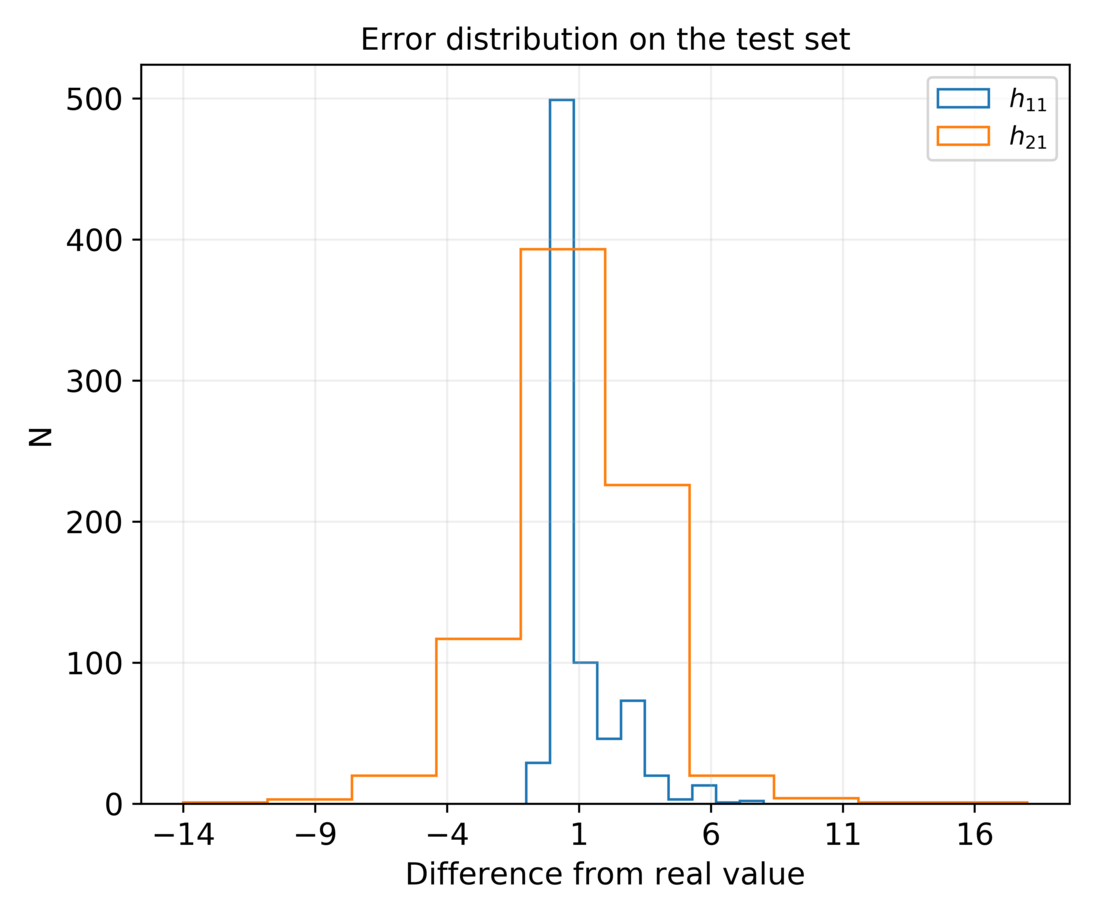
\includegraphics[width=0.75\textwidth]{tex/img/lasso_error_eng.png}
        \caption{Error distribution for \texttt{Lasso} using the engineered dataset.}
        \label{fig:lasso_err}
    \end{figure}
    
\subsection{Ridge Regression}
    We then consider the \texttt{Ridge} algorithm which implements $l2$ regularisation of the fit parameters. We implement a search space for the \texttt{BayesSearchCV} for the hyperparameters \texttt{alpha}, \texttt{fit\_intercept}, \texttt{normalize} and we use the \textit{floor} function for the accuracy.
    
    The naive computation with only the matrix components for $h_{11}$ reached $50.9\% \pm 1.1\%$ of accuracy during cross-validation and $50.0\%$ of accuracy for the test predictions using \texttt{alpha = 3.2}, \texttt{fit\_intercept = False} and \texttt{normalize = True}. The same computation for $h_{21}$ led to $11.5\% \pm 1.3\%$ during cross-validation and $10.3\%$ of accuracy in the test set using \texttt{alpha = $2.5 \times 10^{-2}$}, \texttt{fit\_intercept = True} and \texttt{normalize = True}.
    
    The baseline computation with \texttt{num\_cp} only for $h_{11}$ reached $62\% \pm 2\%$ of accuracy during cross-validation and $63\%$ of accuracy during the test predictions using \texttt{alpha = 100.0}, \texttt{fit\_intercept = True} and \texttt{normalize = False}, thus showing a major improvement in the predictions with respect to the naive case. For $h_{21}$ we find $10.5\% \pm 0.8\%$ of accuracy in cross-validation and $9.8\%$ for the test set using \texttt{alpha = 0.2}, \texttt{fit\_intercept = True} and \texttt{normalize = True}.
    
    The second baseline computation using only \texttt{dim\_cp} shows a worse result for $h_{11}$ with $44\% \pm 2\%$ in cross-validation and $45\%$ of accuracy for the test predictions with \texttt{alpha = 0.18}, \texttt{fit\_intercept = True} and \texttt{normalize = True}, while the results for $h_{21}$ are $8.7\% \pm 1.2\%$ in cross-validation and $9.3\%$ of accuracy for the test set using \texttt{alpha = 99.6}, \texttt{fit\_intercept = False} and \texttt{normalize = False}.
    
    The complete computation using the engineered features does not improve $h_{11}$ but the results for $h_{21}$ get better. Specifically we get $55\% \pm 3\%$ of accuracy in cross-validation for $h_{11}$ and $55\%$ during the test predictions using \texttt{alpha = 99.8}, \texttt{fit\_intercept = True} and \texttt{normalize = False}, while the accuracy for $h_{21}$ is almost doubled with $19.6\% \pm 1.6\%$ of accuracy during cross-validation and $20.1\%$ during the test predictions using \texttt{alpha = 0.39}, \texttt{fit\_intercept = False} and \texttt{normalize = False}. We show in Figure~\ref{fig:ridge_err} the distribution of the the errors of the test predictions.
    
    \begin{figure}[t]
        \centering
        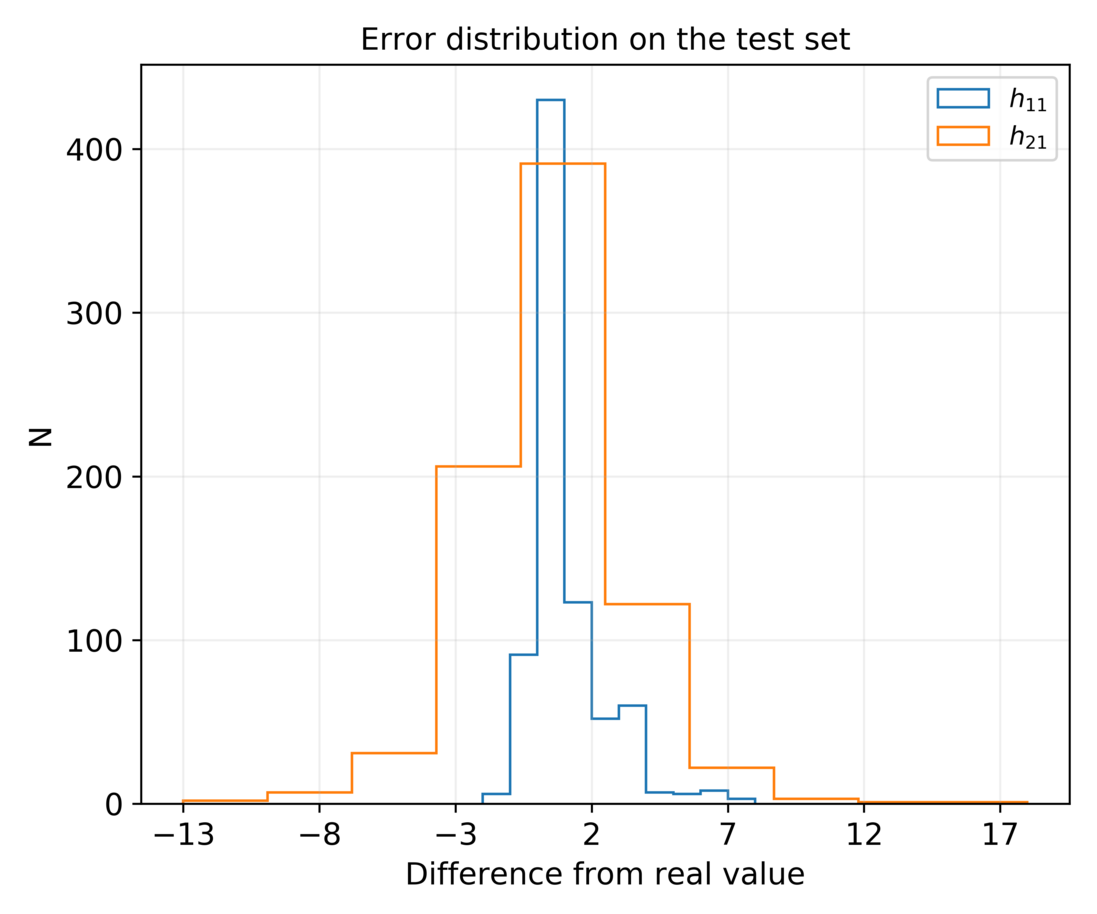
\includegraphics[width=0.75\textwidth]{tex/img/ridge_error_eng.png}
        \caption{Error distribution for \texttt{Ridge} using the engineered dataset.}
        \label{fig:ridge_err}
    \end{figure}
    
\subsection{Elastic Net Regression}
    We then consider the \texttt{ElasticNet} algorithm which implements both $l1$ and $l2$ regularisation. We implement a search space for the \texttt{BayesSearchCV} for the hyperparameters \texttt{alpha}, \texttt{fit\_intercept}, \texttt{l1\_ratio}, \texttt{normalize} and \texttt{positive} and we use the \textit{floor} function for the accuracy.
    
    The naive computation with only the matrix components for $h_{11}$ reached $51.3\% \pm 1.6\%$ of accuracy during cross-validation and $51.0\%$ of accuracy for the test predictions using \texttt{alpha = $3.2 \times 10^{-6}$}, \texttt{fit\_intercept = True}, \texttt{l1\_ratio = 0.0}, \texttt{normalize = True} and \texttt{positive = True}. The same computation for $h_{21}$ led to $11.4\% \pm 1.1\%$ during cross-validation and $13.6\%$ of accuracy in the test set using \texttt{alpha = $1.0 \times 10^{-6}$}, \texttt{fit\_intercept = True}, \texttt{l1\_ratio = 0.15}, \texttt{normalize = True} and \texttt{positive = False}.
    
    The baseline computation with \texttt{num\_cp} only for $h_{11}$ reached $62\% \pm 2\%$ of accuracy during cross-validation and $63\%$ of accuracy during the test predictions using \texttt{alpha = $5.6 \times 10^{-2}$}, \texttt{fit\_intercept = True}, \texttt{l1\_ratio = 0.9}, \texttt{normalize = False} and \texttt{positive = False}, thus showing a major improvement in the predictions with respect to the naive case. For $h_{21}$ we find $12.0\% \pm 0.7\%$ of accuracy in cross-validation and $10.6\%$ for the test set using \texttt{alpha = $6.1 \times 10^{-5}$}, \texttt{fit\_intercept = True}, \texttt{l1\_ratio = 0.005}, \texttt{normalize = True} and \texttt{positive = False}.
    
    The second baseline computation using only \texttt{dim\_cp} shows a worse result for $h_{11}$ with $48\% \pm 2\%$ in cross-validation and $48\%$ of accuracy for the test predictions with \texttt{alpha = $3.9 \times 10^{-5}$}, \texttt{fit\_intercept = True}, \texttt{l1\_ratio = 0.0}, \texttt{normalize = True} and \texttt{positive = True}, while the results for $h_{21}$ are $9.5\% \pm 0.7\%$ in cross-validation and $9.5\%$ of accuracy for the test set using \texttt{alpha = 0.16}, \texttt{fit\_intercept = False}, \texttt{l1\_ratio = 0.0}, \texttt{normalize = False} and \texttt{positive = False}.
    
    The complete computation using the engineered features improves both $h_{11}$ and $h_{21}$. Specifically we get $63\% \pm 2\%$ of accuracy in cross-validation for $h_{11}$ and $64\%$ during the test predictions using \texttt{alpha = 0.07}, \texttt{fit\_intercept = False}, \texttt{l1\_ratio = 1.0}, \texttt{normalize = False} and \texttt{positive = False}, while the accuracy for $h_{21}$ is almost doubled with $19.7\% \pm 1.6\%$ of accuracy during cross-validation and $17.8\%$ during the test predictions using \texttt{alpha = $2.0 \times 10^{-3}$}, \texttt{fit\_intercept = False}, \texttt{l1\_ratio = 0.98}, \texttt{normalize = True} and \texttt{positive = False}. We show in Figure~\ref{fig:el_net_err} the distribution of the the errors of the test predictions.
    
    \begin{figure}[t]
        \centering
        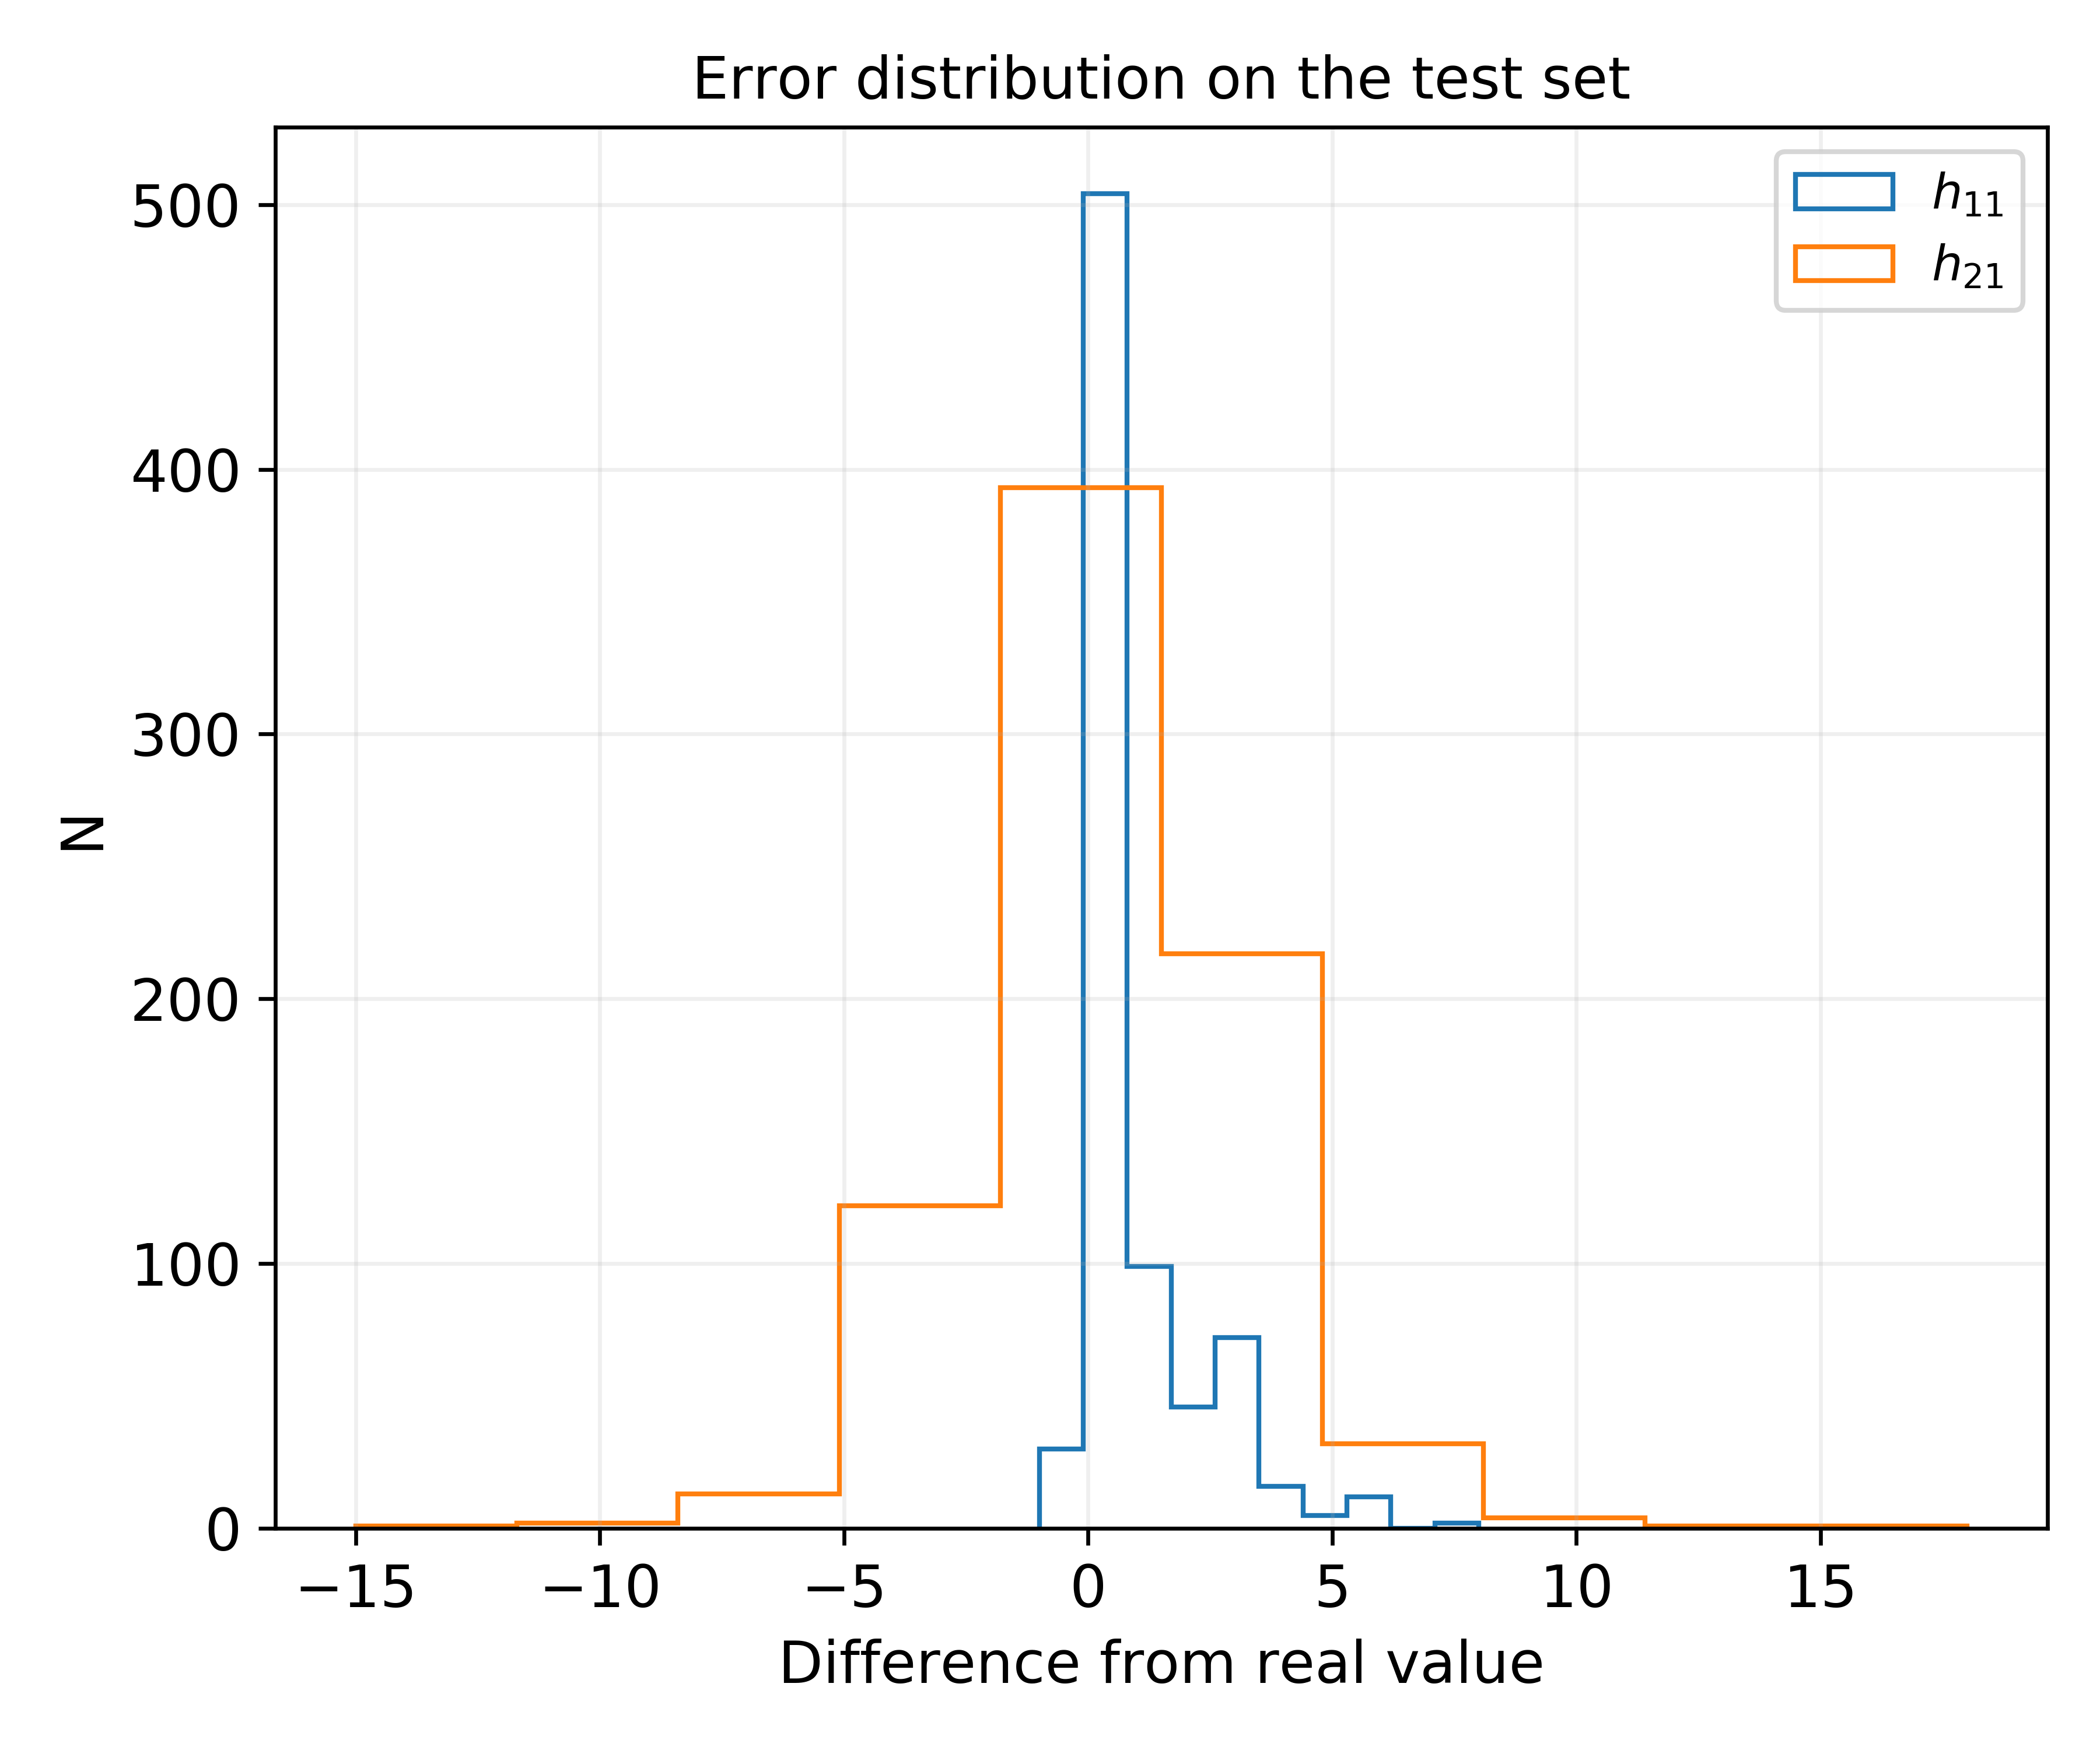
\includegraphics[width=0.75\textwidth]{tex/img/el_net_error_eng.png}
        \caption{Error distribution for \texttt{ElasticNet} using the engineered dataset.}
        \label{fig:el_net_err}
    \end{figure}
    
\subsection{Linear Support Vector}
    We then consider the \texttt{LinearSVR} algorithm. We implement a search space for the \texttt{BayesSearchCV} for the hyperparameters \texttt{C}, \texttt{fit\_intercept}, \texttt{intercept\_scaling} and \texttt{loss} and we use the \textit{floor} function for the accuracy.
    
    The naive computation with only the matrix components for $h_{11}$ reached $51.0\% \pm 1.3\%$ of accuracy during cross-validation and $50.3\%$ of accuracy for the test predictions using  \texttt{C = 0.06}, \texttt{fit\_intercept = True}, \texttt{intercept\_scaling = 100.0} and \texttt{loss = ``squared\_epsilon\_insensitive''}. The same computation for $h_{21}$ led to $11.5\% \pm 1.6\%$ during cross-validation and $8.9\%$ of accuracy in the test set using \texttt{C = 0.010}, \texttt{fit\_intercept = True}, \texttt{intercept\_scaling = 0.01} and \texttt{loss = ``epsilon\_insensitive''}.
    
    The baseline computation with \texttt{num\_cp} only for $h_{11}$ reached $62\% \pm 2\%$ of accuracy during cross-validation and $63\%$ of accuracy during the test predictions using \texttt{C = $4.3 \times 10^{-4}$}, \texttt{fit\_intercept = False}, \texttt{intercept\_scaling = 2.6} and \texttt{loss = ``epsilon\_insensitive''}, thus showing a major improvement in the predictions with respect to the naive case. For $h_{21}$ we find $12.0\% \pm 0.7\%$ of accuracy in cross-validation and $12.3\%$ for the test set using \texttt{C = $1.0 \times 10^{-4}$}, \texttt{fit\_intercept = True}, \texttt{intercept\_scaling = 100.0} and \texttt{loss = ``squared\_epsilon\_insensitive''}.
    
    The second baseline computation using only \texttt{dim\_cp} shows a worse result for $h_{11}$ with $47\% \pm 2\%$ in cross-validation and $50\%$ of accuracy for the test predictions with \texttt{C = 0.19}, \texttt{fit\_intercept = True}, \texttt{intercept\_scaling = 1.29} and \texttt{loss = ``epsilon\_insensitive''}, while the results for $h_{21}$ are $9.5\% \pm 1.1\%$ in cross-validation and $7.3\%$ of accuracy for the test set using \texttt{C = 0.004}, \texttt{fit\_intercept = True}, \texttt{intercept\_scaling = 1.50} and \texttt{loss = ``epsilon\_insensitive''}.
    
    The complete computation using the engineered features improves both $h_{11}$ and $h_{21}$ but shows a slight tendency to overfit for the latter. Specifically we get $62\% \pm 2\%$ of accuracy in cross-validation for $h_{11}$ and $63\%$ during the test predictions using \texttt{C = $1.0 \times 10^{-4}$}, \texttt{fit\_intercept = False}, \texttt{intercept\_scaling = 100.0} and \texttt{loss = ``squared\_epsilon\_insensitive''}, while the accuracy for $h_{21}$ is almost doubled with $21\% \pm 2\%$ of accuracy during cross-validation and $17\%$ during the test predictions using \texttt{C = 0.4}, \texttt{fit\_intercept = True}, \texttt{intercept\_scaling = 100.0} and \texttt{loss = ``epsilon\_insensitive''}. We show in Figure~\ref{fig:lin_svr_err} the distribution of the the errors of the test predictions.
    
    \begin{figure}[t]
        \centering
        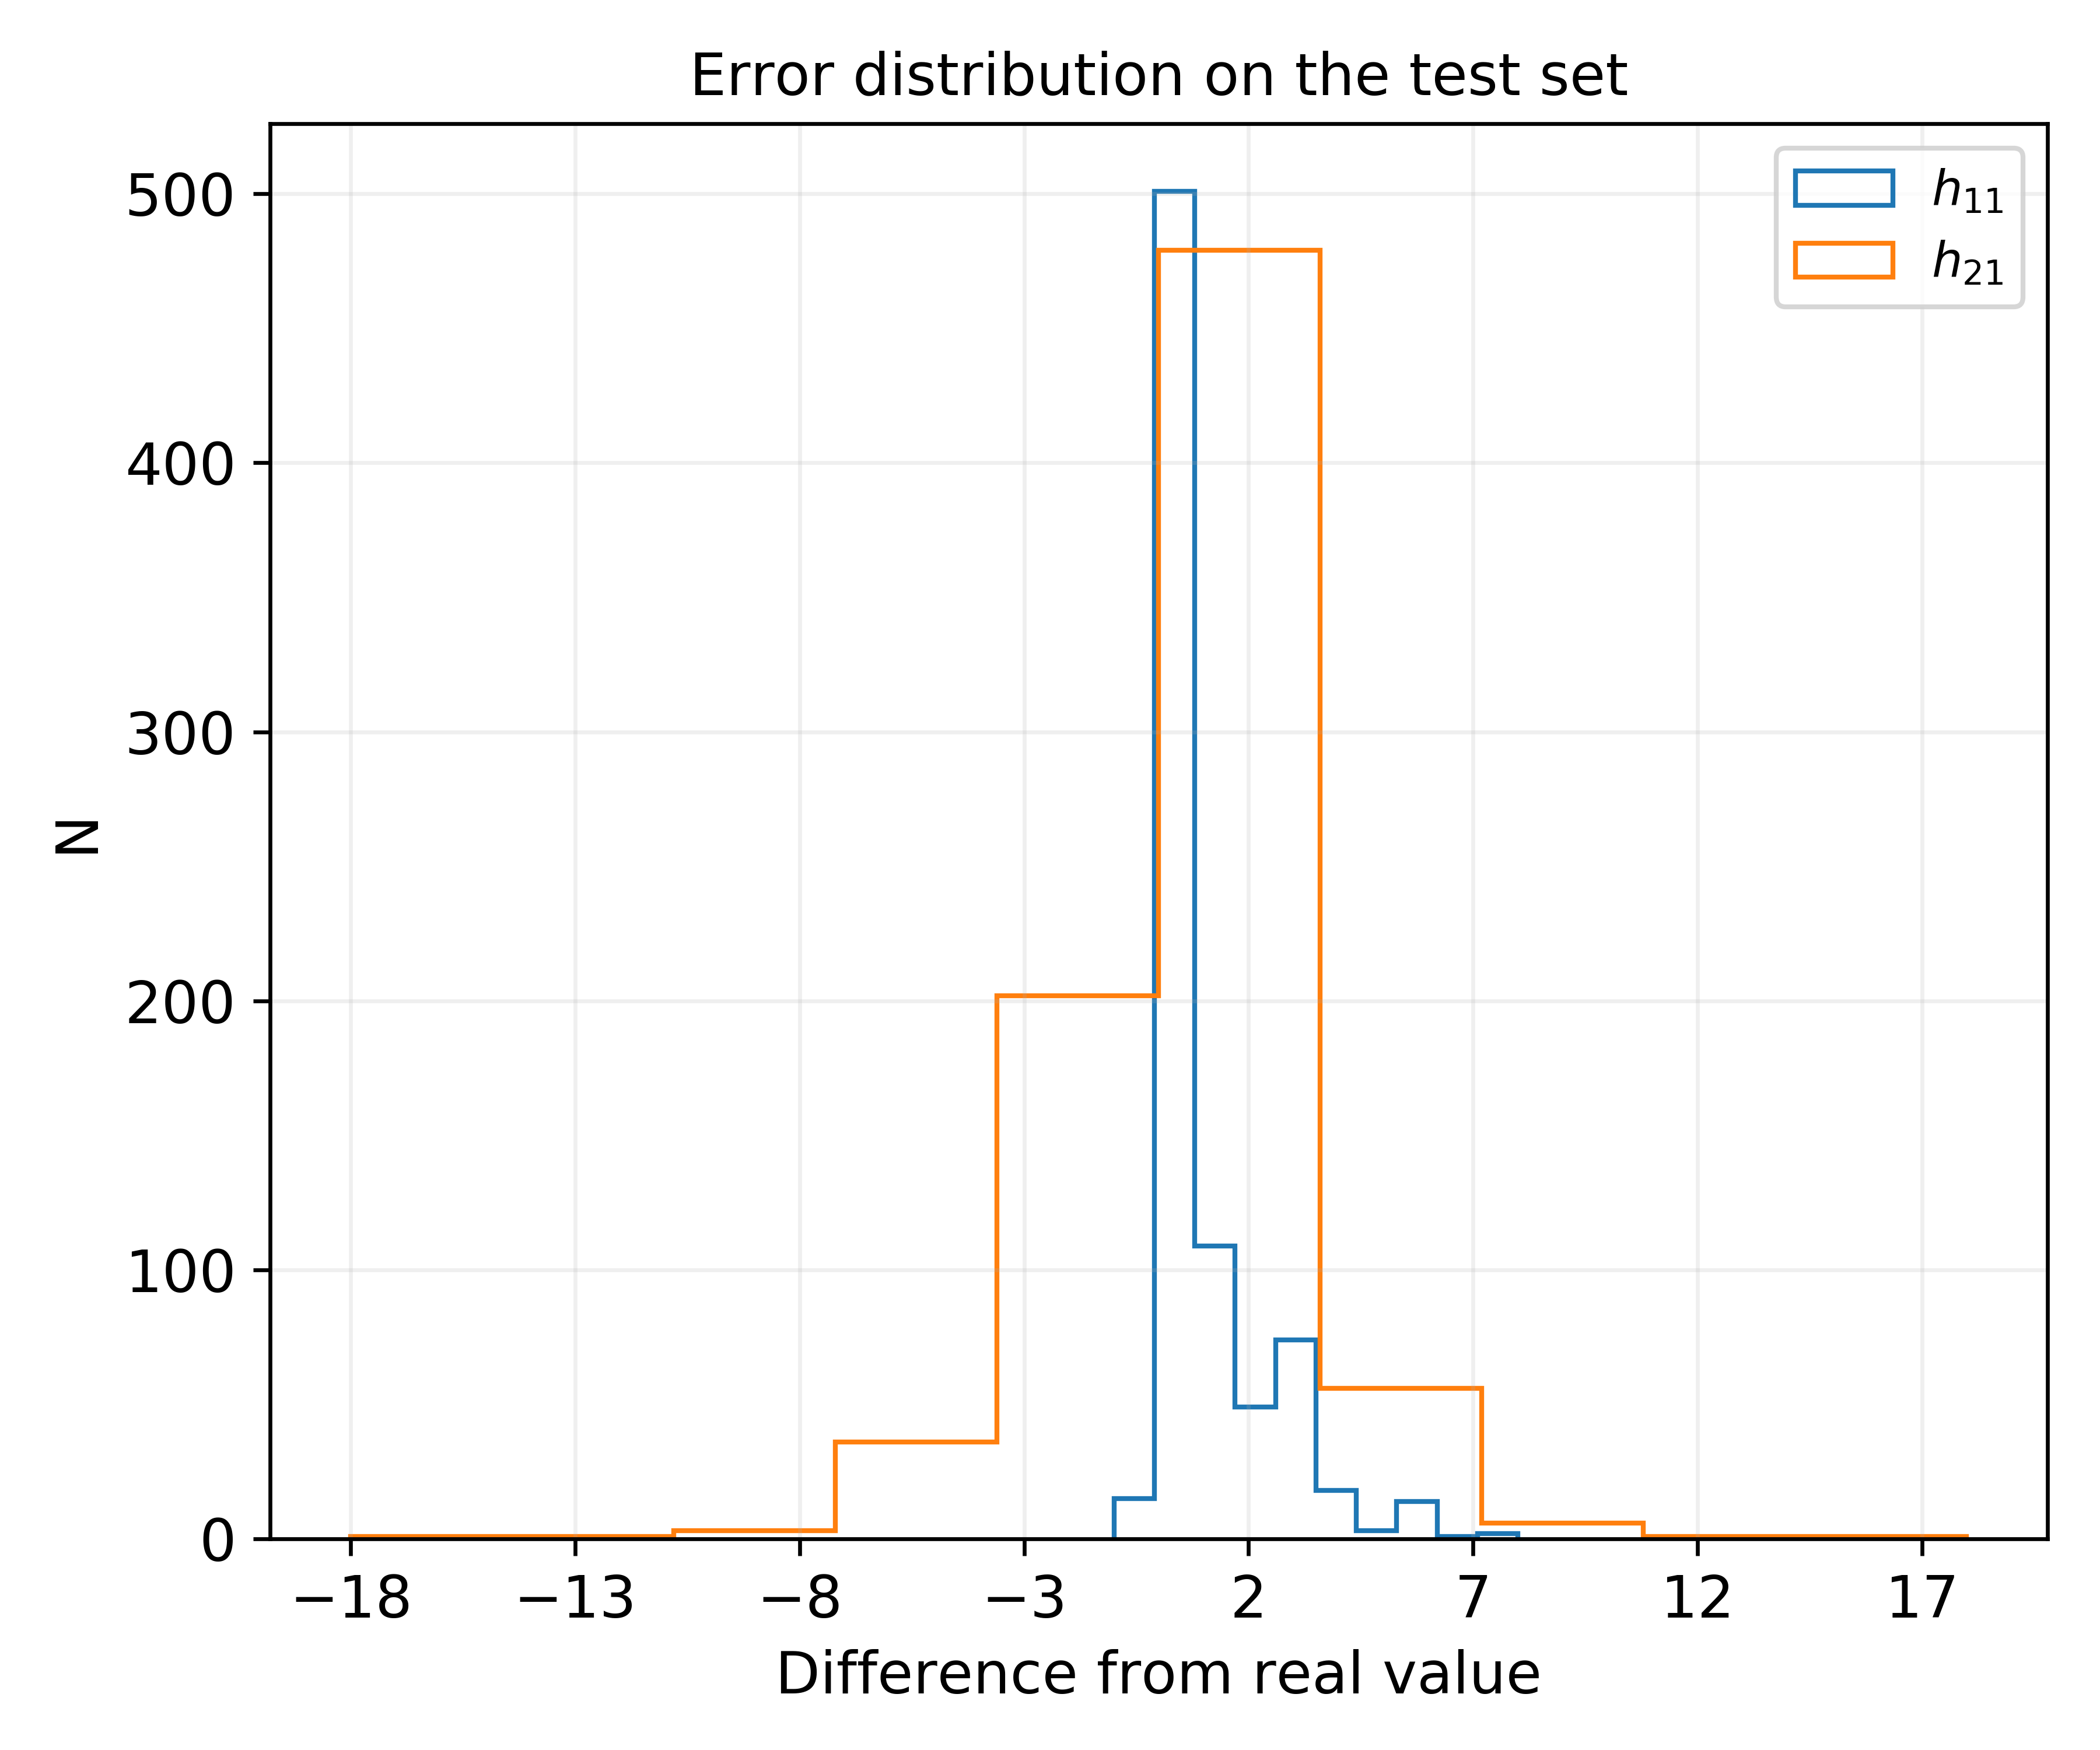
\includegraphics[width=0.75\textwidth]{tex/img/lin_svr_error_eng.png}
        \caption{Error distribution for \texttt{LinearSVR} using the engineered dataset.}
        \label{fig:lin_svr_err}
    \end{figure}
    
\subsection{Gaussian Support Vector}
    We then consider the \texttt{SVR} algorithm with \textit{rbf} kernel. We implement a search space for the \texttt{BayesSearchCV} for the hyperparameters \texttt{C}, \texttt{epsilon}, \texttt{gamma} and \texttt{shrinking} and we use the \textit{rint} function for the accuracy.
    
    The naive computation with only the matrix components for $h_{11}$ reached $70\% \pm 2\%$ of accuracy during cross-validation and $69\%$ of accuracy for the test predictions using \texttt{C = 6.3}, \texttt{epsilon = $1.0 \times 10^{-5}$}, \texttt{gamma = 0.06} and \texttt{shrinking = True}. The same computation for $h_{21}$ led to $22\% \pm 2\%$ during cross-validation and $21\%$ of accuracy in the test set using \texttt{C = 15.0}, \texttt{epsilon = $1.0 \times 10^{-5}$}, \texttt{gamma = 0.10} and \texttt{shrinking = True}.
    
    The baseline computation with \texttt{num\_cp} only for $h_{11}$ reached $62\% \pm 2\%$ of accuracy during cross-validation and $63\%$ of accuracy during the test predictions using \texttt{C = 0.70}, \texttt{epsilon = $1.0 \times 10^{-5}$}, \texttt{gamma = $1.0 \times 10^{-6}$} and \texttt{shrinking = False}, showing a slight worsening with respect to the naive case. For $h_{21}$ we find $11.9\% \pm 0.9\%$ of accuracy in cross-validation and $12.3\%$ for the test set using \texttt{C = $1.0 \times 10^{4}$}, \texttt{epsilon = $1.0 \times 10^{-5}$}, \texttt{gamma = $1.0 \times 10^{-6}$} and \texttt{shrinking = True}.
    
    The second baseline computation using only \texttt{dim\_cp} shows a small improvement for $h_{11}$ with $65\% \pm 2\%$ in cross-validation and $68\%$ of accuracy for the test predictions with \texttt{C = 155}, \texttt{epsilon = $4.8 \times 10^{-4}$}, \texttt{gamma = 0.02} and \texttt{shrinking = False}, while the results for $h_{21}$ are $14.7\% \pm 1.2\%$ of accuracy in cross-validation and $15.3\%$ for the test set using \texttt{C = 1320}, \texttt{epsilon = $1.0 \times 10^{-5}$}, \texttt{gamma = 100.0} and \texttt{shrinking = True}.
    
    The complete computation using the engineered features improves both $h_{11}$ and $h_{21}$ and represents the best result of the machine learning analysis (neural networks excluded). Specifically we get $71\% \pm 2\%$ of accuracy in cross-validation for $h_{11}$ and $72\%$ during the test predictions using \texttt{C = 1.3}, \texttt{epsilon = $3.4 \times 10^{-4}$}, \texttt{gamma = 0.02} and \texttt{shrinking = False}, while the accuracy for $h_{21}$ is almost doubled with $37.0\% \pm 1.6\%$ of accuracy during cross-validation and $37.2\%$ during the test predictions using \texttt{C = 24.6}, \texttt{epsilon = $4.0 \times 10^{-5}$}, \texttt{gamma = 0.007} and \texttt{shrinking = False}. We show in Figure~\ref{fig:svr_rbf_err} the distribution of the the errors of the test predictions.
    
    \begin{figure}[t]
        \centering
        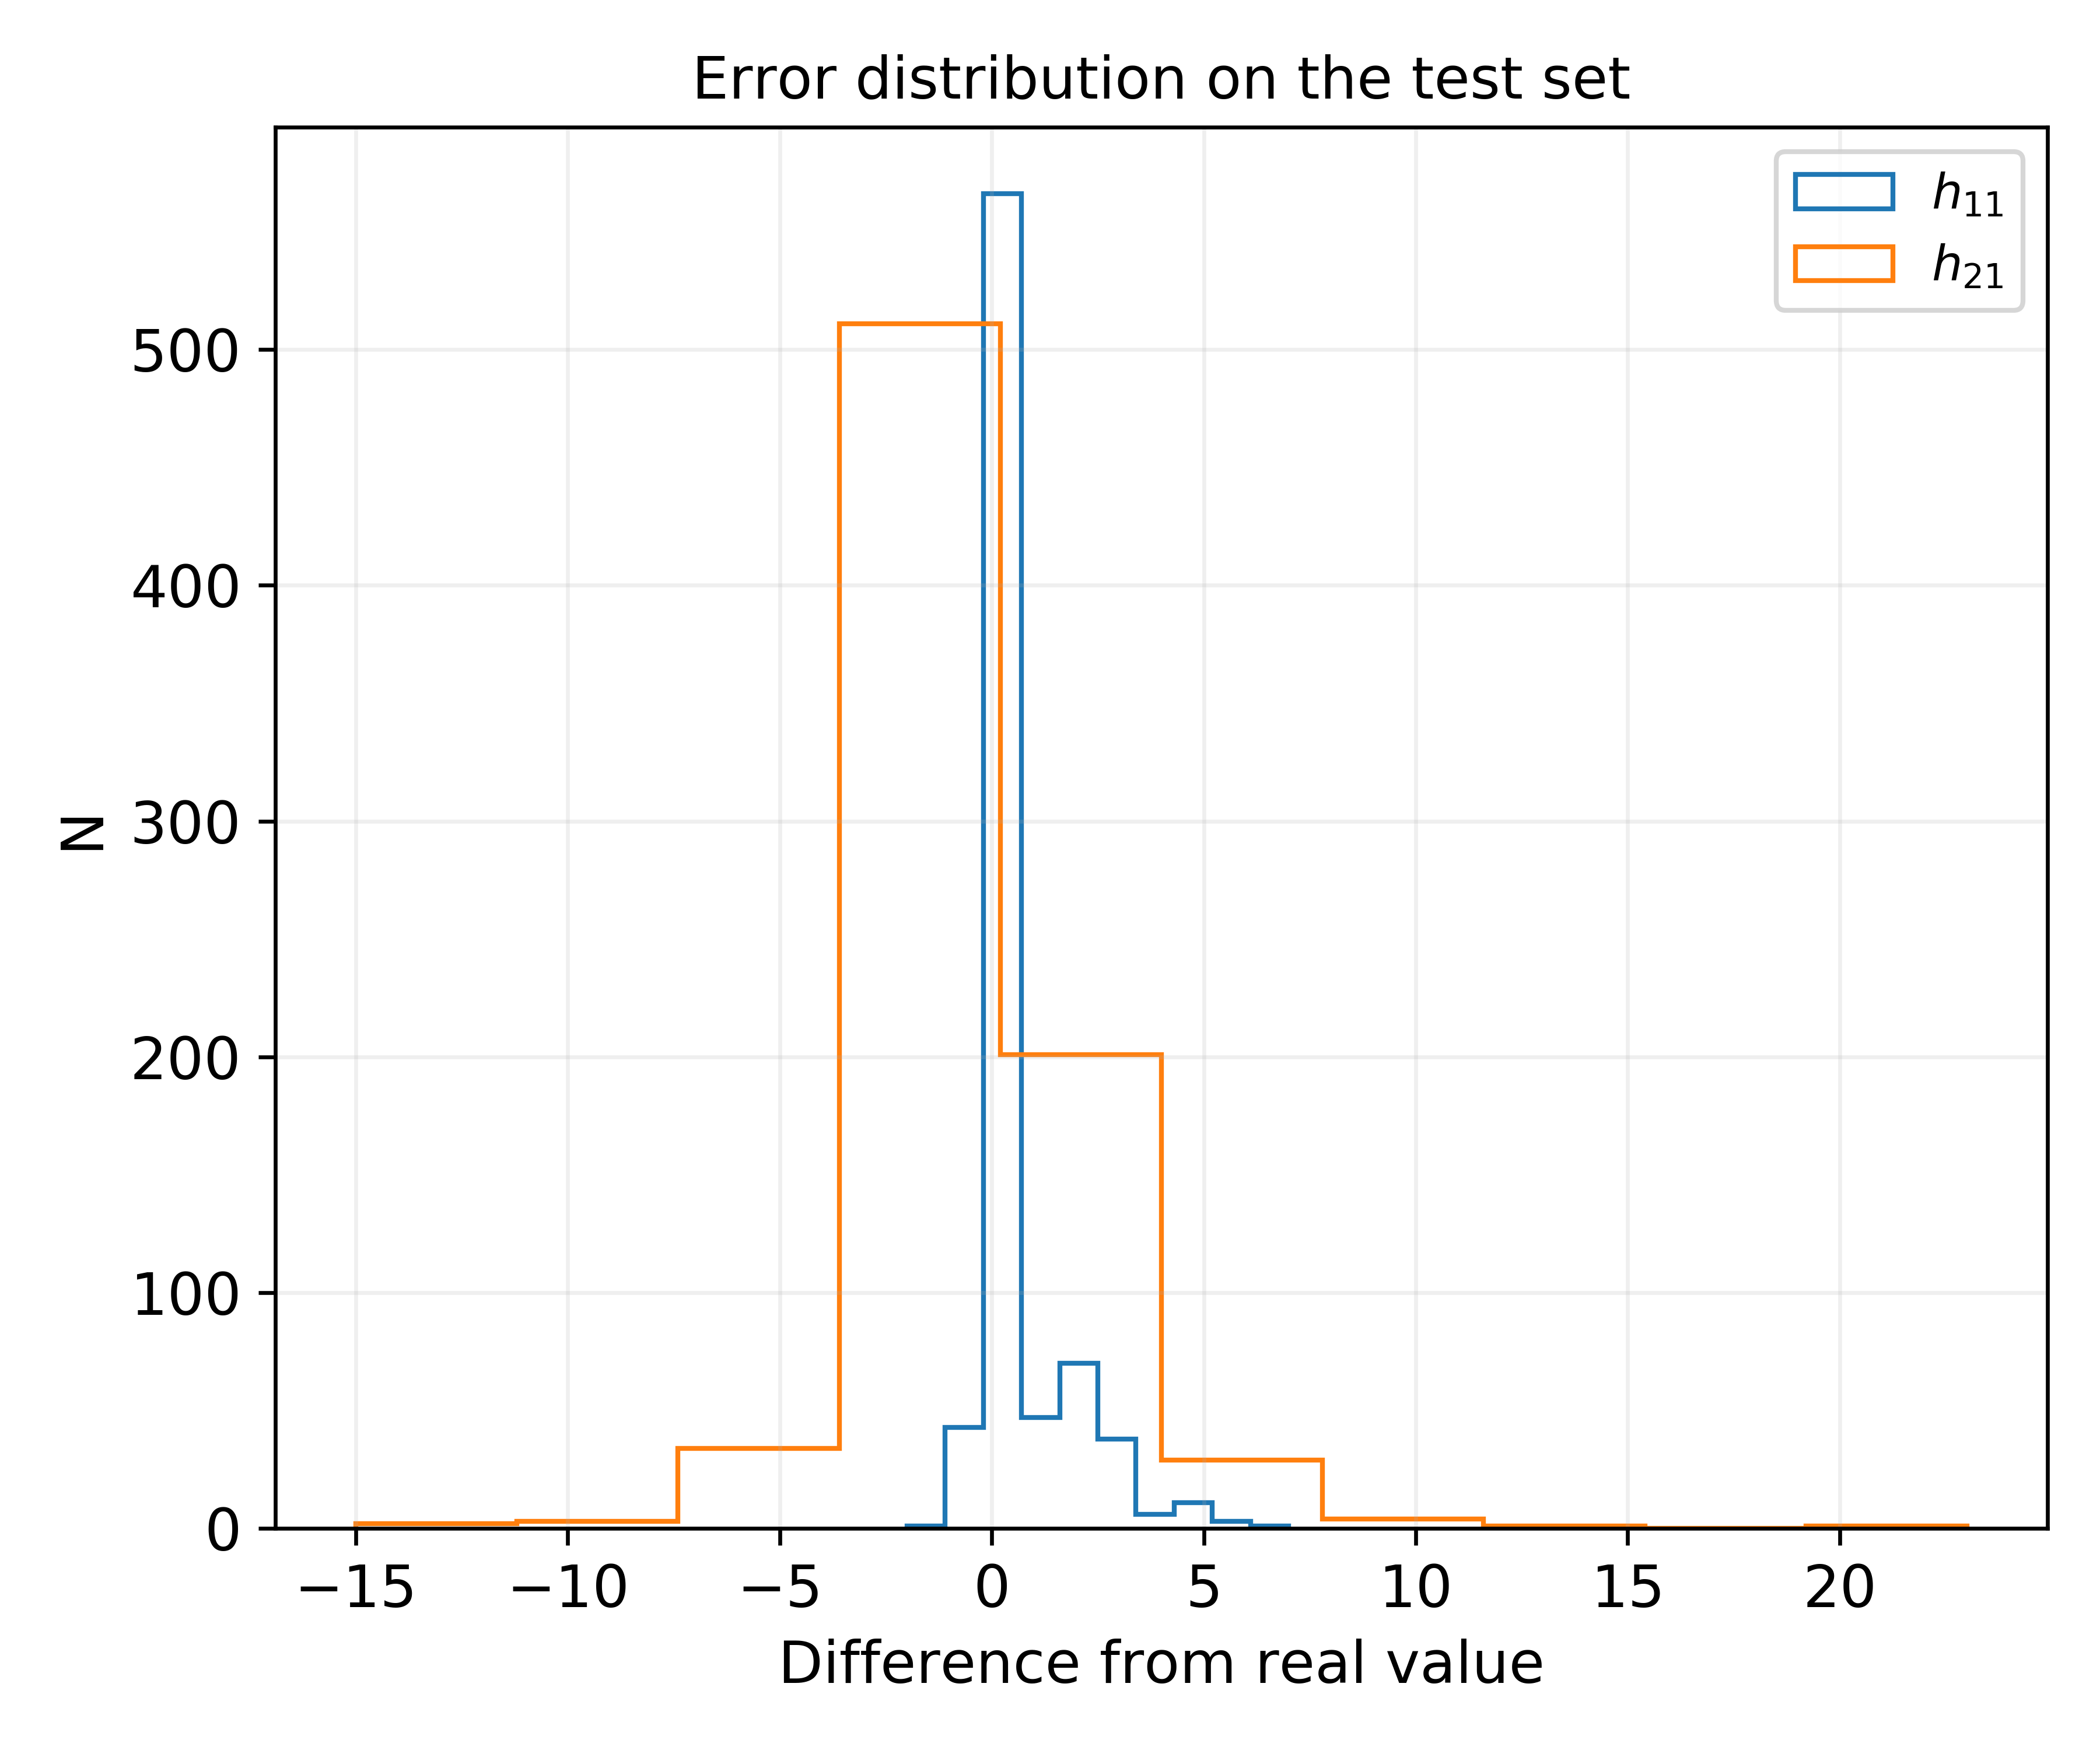
\includegraphics[width=0.75\textwidth]{tex/img/svr_rbf_error_eng.png}
        \caption{Error distribution for \texttt{SVR} with \textit{rbf} kernel using the engineered dataset.}
        \label{fig:svr_rbf_err}
    \end{figure}